%  Architecture.tex
%  Document created by seblovett on octopus
%  Date created: Wed 02 Apr 2014 14:03:33 BST
%  <+Last Edited: Wed 02 Apr 2014 14:47:11 BST by hl13g10 on octopus +>

\section{Architecture}

Discuss the overall architecture

A register-accumulator based architecture was decided to be used. 
This results in the instruction only needing one operand, reducing the overall size. 
Figure \ref{fig:arch} shows the architecture of the processor, excluding the control and control signals.

\begin{figure}
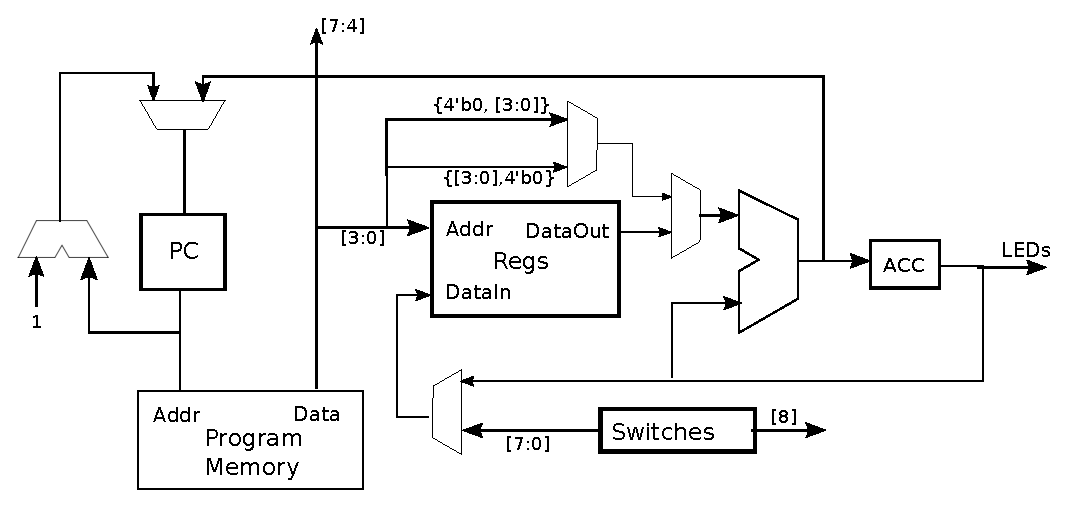
\includegraphics[width=\textwidth]{Figures/architecture.eps}
\caption{Block Diagram of the architecture. Control unit and signals have been omitted for clarity.}
\label{fig:arch}
\end{figure}

Each aspect of the processor are discussed in the following sections, looking at the design, test and synthesis of the modules.
